% Ergebnisse


%\chapter{Ergebnisse}
\section{Ergebnisse}
\label{ergebnisse}

\todo{Eigenes kapitel? P}

Das Ergebnis der Implementierung ist eine aus mehreren \textit{Unity} Szenen bestehendes \textit{Unity} Projekt.
Die Vr- und AR-Anwendungen bestehen jeweils aus zwei Szenen, eine für die zwei-, eine für die dreidimensionale Darstellung sowie einer Startszene Preload.unity, in der ein GameObject namens appState liegt, über das bestimmt werden kann, welche Szene zuerst geladen werden soll. In diesem Objekt werden auch die Zustände der Szenen gespeichert und so Manipulationen übertragen.
Die Szenen für die 2D-Darstellung heißen main\_2D.unity und main\_2D\_AR.unity. Die für die 3D-Darstellung main\_3D.unity und main\_3D\_AR.unity.

Die VR-Anwendung ist als ausführbare Datei im Ergänzungsmaterial zu finden. Da die \textit{HoloLens}-Anwendung, wie in Kapitel \ref{konzept} erläutert, nicht für diese bereitgestellt werden konnte, existiert hierfür keine ausführbare Datei. Allerdings wurde in der ReadMe.txt Datei des Projektes, die sich ebenfalls im Ergänzungsmaterial beschrieben, wie die Anwendung auf der \textit{HoloLens} abgespielt werden kann. 
Weiterhin ist dort zwei Videos enthalten, die die Funktionen und Bedienung der Anwendung zeigen.

Die Interaktionslemente wurden bereits in Kapitel \ref{konzept} beschrieben und abgebildet. 
Screenshots
beschreibung der Anwendung

\subsection{3D Darstellung}

In Kapitel \ref{implementierung} wurde erläutert, wie die 3D-Darstellung mit Hilfe von Volume Raycasting erzeugt wurde. 
Dazu wurde der Alphawert einer Transfertextur genutzt, um das Rauschen in der Umgebung des Gehirns zu entfernen und die Gehirnform eindeutiger herauszustellen. Dies führt allerdings auch zu Artefakten, dem sogenannten Holzmaserungseffekt. Da allerdings die Darstellung der inneren Strukturen des Gehirns im Vordergrund steht, wurde sich für eine Darstellung entschieden, die durch Reduzierung der Umgebung den Fokus auf das Gehirn erlaubt. 
Im Abbildung \ref{img:results} sind die beiden Datensätze mit und ohne die Verwendung einer Transferfunktion abgebildet. 
Es ist anzumerken, dass die Qualität der Daten sich unweigerlich auf die Qualität des Renderings auswirkt. Die vorgegebenen Datensätze des Gehirns wiesen ein hohes Maß an Bildrauschen auf. Außerdem wurden die Schichten offenbar in in Abständen solcher Größe gescannt, dass die Interpolation zwischen den Schichten Aktefakte ausweist. Auch dies in in Abbildung \ref{img:results} zu sehen.

\begin{figure}[!htb]
	\centering
	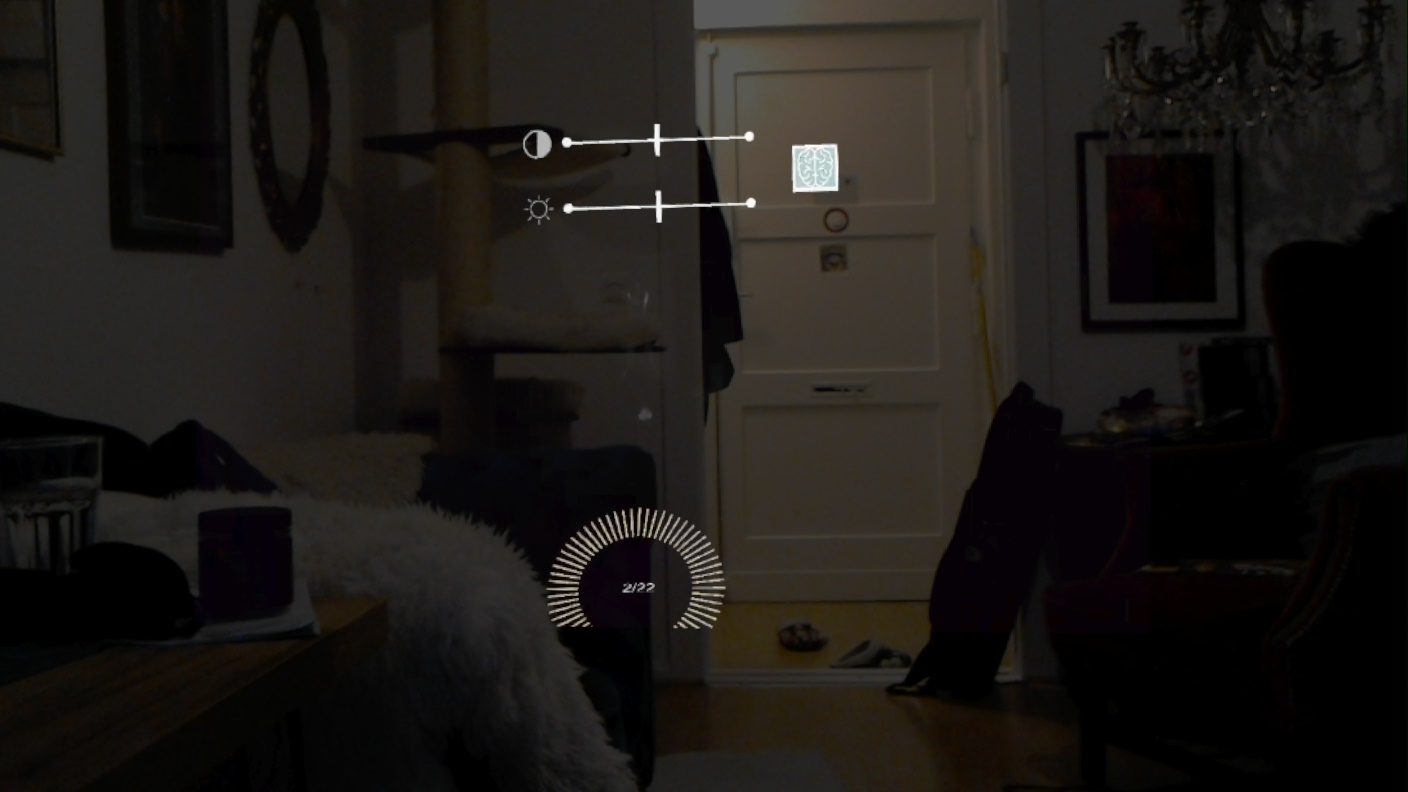
\includegraphics[width=0.5\linewidth]{images/hololens2D.jpg}
	\caption{Rendering der zur Verfügung gestellten Datensätze durch den in mARt verwendeten Shader. a) Datensatz 1 ohne Transferfunktion, Intensität: XY. b) Datensatz 1 mit Transferfunktion, Intensität: XY. c) Datensatz 2 ohne Transferfunktion, Intensität: XY d) Datensatz 2 mit Transferfunktion, Intensität: XY}
	\label{img:result}
	\source{Eigene Darstellung}
\end{figure}
\FloatBarrier
  
Aus diesem Grund wurden testweise auch andere Daten mit dem selben Shader gerendert. Das Ergebnis ist dabei von besserer Qualität als mit den Gehirndaten. Die Verwendung der Transferfunktion ist nicht notwendig, um die Darstellung deutlicher zu machen. Durch Manipulation der Intensität kann bestimmt werden, in welcher Tiefe das Gewebe gerendert werden soll. In Abbildung \ref{img:resultsVisMale} ist der Datensatz eines Kopfes mit und ohne sowie mit verschiedener Intensität dargestellt.
  
\begin{figure}[!htb]
	\centering
	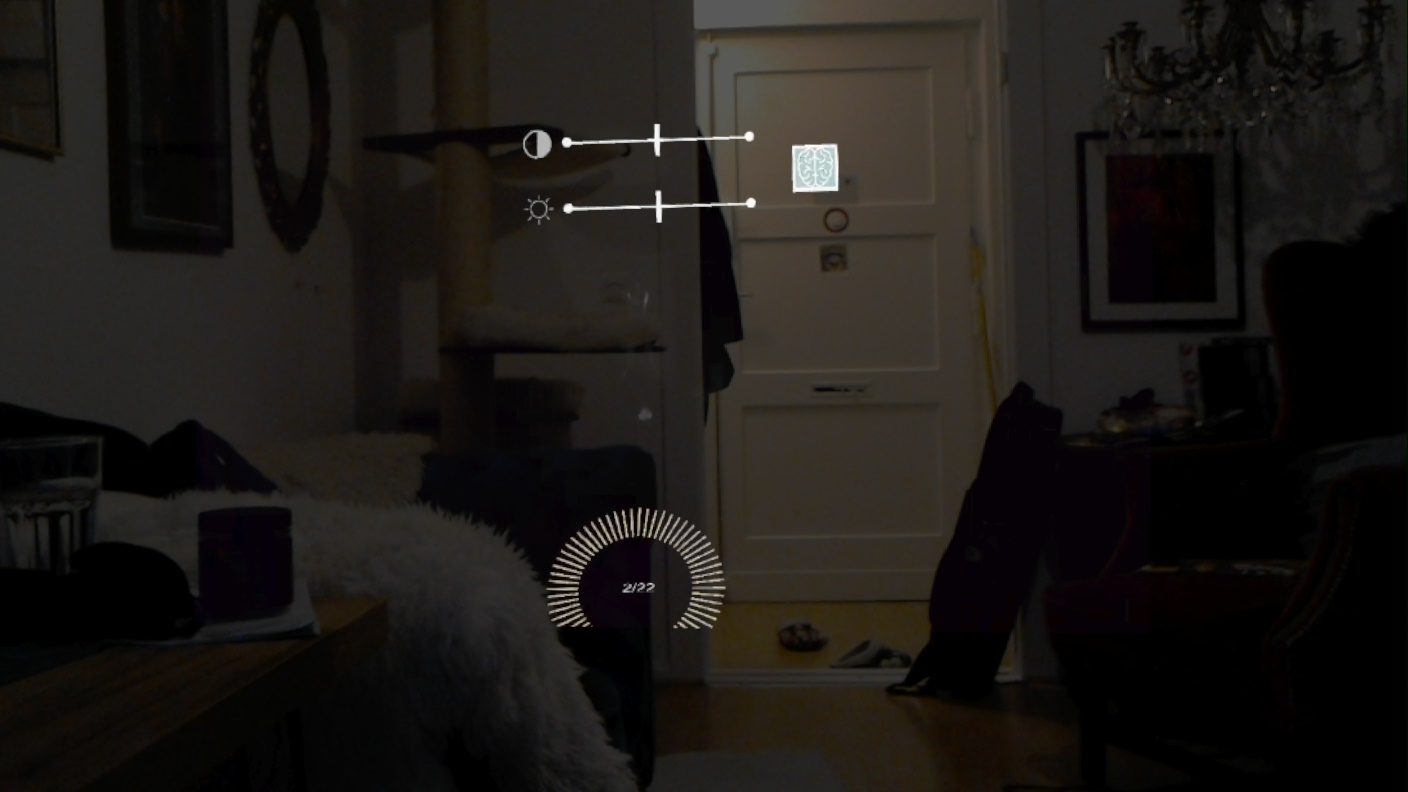
\includegraphics[width=0.5\linewidth]{images/hololens2D.jpg}
	\caption{Rendering eines alternativen Datensatzes durch den in mARt verwendeten Shader. a) Rendering ohne Transferfunktion, Intensität: XY. b) Rendering mit Transferfunktion, Intensität: XY. c) Rendering ohne Transferfunktion, Intensität: yZ.}
	\label{img:resultsVisMale}
	\source{Eigene Darstellung}
\end{figure}
\FloatBarrier
  
\subsection{AR Anwendung}
Durch die semi-transparente Darstellung in AR sind die eher dunklen MRT-Daten teilweise schlecht zu erkennen. Dies betrifft vor allem die 3D-Darstellung. Wie deutlich die Visualisierung ist, hängt von den Lichtverhältnissen ab. In Abbildung \ref{img:ARLicht} ist zu erkennen, wie undeutlich die Daten dargestellt werden und außerdem, wie sich die Helligkeit der Umgebung auf die Darstellung auswirkt. (Abbildung AR?)

-> Artefakte in abhängigkeit zu Daten setzen. \ref{Konzept}

\todo{Bild austauschen}
\begin{figure}[!htb]
	\centering
	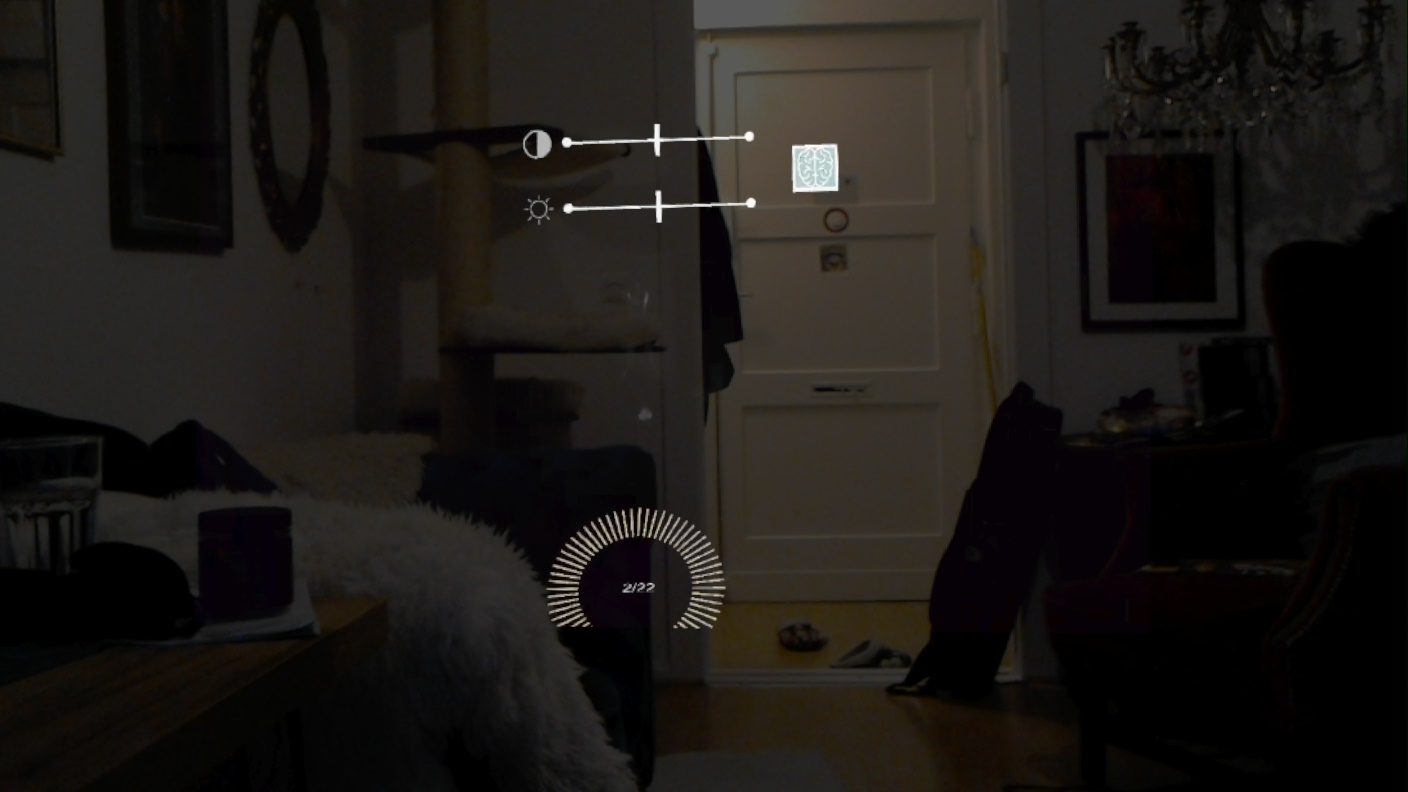
\includegraphics[width=0.5\linewidth]{images/hololens2D.jpg}
	\caption{Eine Aufnahme aus der \textit{HoloLens}, während die 2D-Scene von mARt dargestellt wird in einem eher dunklen Raum. Die Interaktionselemente sind gut zu erkennen, die MRT-Bilder nicht.}
	\label{img:ARLicht}
	\source{Eigene Darstellung}
\end{figure}
\FloatBarrier

Ein weiterer Punkt, der die Verwendung der Anwendung auf der \textit{HoloLens} erschwert ist das eingeschränkte Sichtfeld des Gerätes. Dieses Problem wurde bereit in Kapitel \ref{grundlagen} beschrieben. 
Die Begrenzung der Darstellung führt dazu, dass die MRT-Daten aus der Sicht des Nutzers meist abgeschnitten sind. Um die Daten gleichzeitig mit den Interaktionselementen sehen zu können, muss der Nutzer einen Abstand von ca. 1,5m zur Darstellung haben. Dies macht es ihm allerdings unmöglich mit dieser zu interagieren. Um die Darstellung manipulieren zu können, muss er also zwischen MRT-Bildern und Bedienelementen hin- und herblicken. Dabei werden die virtuellen Hände des Nutzer nicht angezeigt, wenn er diese nicht direkt ansieht, auch wenn die Leap Motion diese vielleicht noch erfasst. 
Die Darstellung der Hände selbst nimmt bereits einen großen Teil des Sichtfeldes der \textit{HoloLens} ein, da sie sich nahe am HMD befinden. 
Eine Bedienung der Anwendung auf der \textit{HoloLens} ist aus diesen Gründen sehr schwer. 


